

\tikzset{every picture/.style={line width=0.75pt}} %set default line width to 0.75pt        

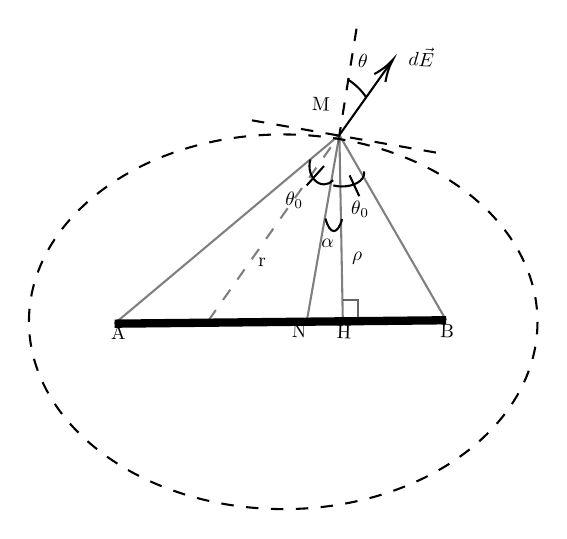
\begin{tikzpicture}[x=0.75pt,y=0.75pt,yscale=-1,xscale=1]
%uncomment if require: \path (0,329); %set diagram left start at 0, and has height of 329

%Shape: Boxed Line [id:dp18134862073246527] 
\draw [color={rgb, 255:red, 0; green, 0; blue, 0 }  ,draw opacity=0.5 ]   (157.09,187.11) -- (265.42,96.21) ;
%Shape: Boxed Line [id:dp12099064274809379] 
\draw [color={rgb, 255:red, 0; green, 0; blue, 0 }  ,draw opacity=0.5 ]   (265.42,96.21) -- (316.85,185.46) ;
%Shape: Boxed Line [id:dp20049333748183473] 
\draw [color={rgb, 255:red, 0; green, 0; blue, 0 }  ,draw opacity=0.5 ]   (265.42,96.21) -- (249.65,186.26) ;
%Shape: Boxed Line [id:dp17865478996636575] 
\draw [color={rgb, 255:red, 0; green, 0; blue, 0 }  ,draw opacity=1 ][line width=3]    (157.09,187.11) -- (316.85,185.46) ;
%Straight Lines [id:da8125496874210176] 
\draw [color={rgb, 255:red, 0; green, 0; blue, 0 }  ,draw opacity=0.5 ] [dash pattern={on 4.5pt off 4.5pt}]  (202.45,185.46) -- (265.42,96.21) ;
%Straight Lines [id:da6002158392672337] 
\draw    (265.42,96.21) -- (290.1,61.49) ;
\draw [shift={(291.25,59.86)}, rotate = 125.4] [color={rgb, 255:red, 0; green, 0; blue, 0 }  ][line width=0.75]    (10.93,-3.29) .. controls (6.95,-1.4) and (3.31,-0.3) .. (0,0) .. controls (3.31,0.3) and (6.95,1.4) .. (10.93,3.29)   ;
%Straight Lines [id:da8906366441589808] 
\draw  [dash pattern={on 4.5pt off 4.5pt}]  (273.67,45) -- (265.42,96.21) ;
%Shape: Boxed Line [id:dp4280899838487169] 
\draw  [dash pattern={on 4.5pt off 4.5pt}]  (311.93,104.67) -- (221.88,88.9) ;
%Shape: Arc [id:dp1052035780036713] 
\draw  [draw opacity=0] (269.36,69.39) .. controls (272.88,71.58) and (275.96,74.51) .. (278.34,78.03) -- (253.48,94.84) -- cycle ; \draw   (269.36,69.39) .. controls (272.88,71.58) and (275.96,74.51) .. (278.34,78.03) ;  
%Shape: Boxed Line [id:dp6660278877118841] 
\draw [color={rgb, 255:red, 0; green, 0; blue, 0 }  ,draw opacity=0.5 ]   (265.42,96.21) -- (267.05,184.66) ;
%Shape: Ellipse [id:dp9767305005316875] 
\draw  [dash pattern={on 4.5pt off 4.5pt}] (115.85,185.92) .. controls (115.96,136.07) and (170.9,95.78) .. (238.56,95.94) .. controls (306.22,96.09) and (360.98,136.62) .. (360.86,186.47) .. controls (360.75,236.32) and (305.81,276.6) .. (238.15,276.45) .. controls (170.49,276.3) and (115.74,235.76) .. (115.85,185.92) -- cycle ;
%Shape: Arc [id:dp6554054937575013] 
\draw  [draw opacity=0] (262.42,118.01) .. controls (261.22,119.26) and (259.68,120) .. (258,120) .. controls (254.13,120) and (251,116.05) .. (251,111.17) .. controls (251,110.07) and (251.16,109.02) .. (251.45,108.06) -- (258,111.17) -- cycle ; \draw   (262.42,118.01) .. controls (261.22,119.26) and (259.68,120) .. (258,120) .. controls (254.13,120) and (251,116.05) .. (251,111.17) .. controls (251,110.07) and (251.16,109.02) .. (251.45,108.06) ;  
%Shape: Arc [id:dp556244560380825] 
\draw  [draw opacity=0] (277.25,113.73) .. controls (277.32,114.03) and (277.35,114.33) .. (277.35,114.64) .. controls (277.35,118.16) and (272.58,121.01) .. (266.69,121.01) .. controls (265.2,121.01) and (263.79,120.83) .. (262.5,120.5) -- (266.69,114.64) -- cycle ; \draw   (277.25,113.73) .. controls (277.32,114.03) and (277.35,114.33) .. (277.35,114.64) .. controls (277.35,118.16) and (272.58,121.01) .. (266.69,121.01) .. controls (265.2,121.01) and (263.79,120.83) .. (262.5,120.5) ;  
%Shape: Right Angle [id:dp627154132195284] 
\draw  [color={rgb, 255:red, 0; green, 0; blue, 0 }  ,draw opacity=0.6 ] (267.05,175.66) -- (274.55,175.66) -- (274.55,184.66) ;
%Shape: Arc [id:dp2502467223266438] 
\draw  [draw opacity=0] (266.73,136.68) .. controls (265.77,140.24) and (264.34,142.5) .. (262.75,142.5) .. controls (261.13,142.5) and (259.68,140.15) .. (258.71,136.46) -- (262.75,125.75) -- cycle ; \draw   (266.73,136.68) .. controls (265.77,140.24) and (264.34,142.5) .. (262.75,142.5) .. controls (261.13,142.5) and (259.68,140.15) .. (258.71,136.46) ;  
%Straight Lines [id:da42998185574073755] 
\draw    (258,111.17) -- (249.67,120.5) ;
%Straight Lines [id:da6176729001517964] 
\draw    (270.33,115.67) -- (275,125.67) ;

% Text Node
\draw (251.36,76.74) node [anchor=north west][inner sep=0.75pt]  [rotate=-2,xscale=0.7,yscale=0.7] [align=left] {M};
% Text Node
\draw (154.39,187.16) node [anchor=north west][inner sep=0.75pt]  [xscale=0.7,yscale=0.7] [align=left] {A};
% Text Node
\draw (313.19,186.29) node [anchor=north west][inner sep=0.75pt]  [rotate=-2,xscale=0.7,yscale=0.7] [align=left] {B};
% Text Node
\draw (241.69,186.1) node [anchor=north west][inner sep=0.75pt]  [rotate=-2,xscale=0.7,yscale=0.7] [align=left] {N};
% Text Node
\draw (273.56,56.07) node [anchor=north west][inner sep=0.75pt]  [rotate=-2,xscale=0.7,yscale=0.7] [align=left] {$\displaystyle \theta $};
% Text Node
\draw (297.98,52.8) node [anchor=north west][inner sep=0.75pt]  [rotate=-2,xscale=0.7,yscale=0.7] [align=left] {$\displaystyle d\vec{E}$};
% Text Node
\draw (263.36,186.94) node [anchor=north west][inner sep=0.75pt]  [rotate=-2,xscale=0.7,yscale=0.7] [align=left] {H};
% Text Node
\draw (225.35,154.47) node [anchor=north west][inner sep=0.75pt]  [rotate=-2,xscale=0.7,yscale=0.7] [align=left] {r};
% Text Node
\draw (238.33,122.5) node [anchor=north west][inner sep=0.75pt]  [xscale=0.7,yscale=0.7] [align=left] {$\displaystyle \theta _{0}$};
% Text Node
\draw (270.05,127.04) node [anchor=north west][inner sep=0.75pt]  [xscale=0.7,yscale=0.7] [align=left] {$\displaystyle \theta _{0}$};
% Text Node
\draw (270.5,151.5) node [anchor=north west][inner sep=0.75pt]  [xscale=0.7,yscale=0.7] [align=left] {$\displaystyle \rho $};
% Text Node
\draw (255.67,145.33) node [anchor=north west][inner sep=0.75pt]  [xscale=0.7,yscale=0.7] [align=left] {$\displaystyle \alpha $};


\end{tikzpicture}